\begin{enumerate}[label=\thesubsection.\arabic*.,ref=\thesubsection.\theenumi]

\numberwithin{equation}{enumi}
\numberwithin{figure}{enumi}


\item 
8-PSK 
Consider
\begin{align}
\textbf{y = s + n}
\end{align}

where \textbf{ s$\in$ \{$s_0$, $s_1$, $s_2$, $s_3$,$s_4$,$s_5$,$s_6$,$s_7$\}}

\begin{align}
    s_0 = 
    \begin{pmatrix}
     \sqrt{E_s} \\
     0
    \end{pmatrix}
\end{align}

\begin{align}
    s_1 = 
    \begin{pmatrix}
     \sqrt{\frac{E_s}{2}}\\
     \sqrt{\frac{E_s}{2}}
    \end{pmatrix}
\end{align}
\begin{align}
    s_2 = 
    \begin{pmatrix}
      0 \\
     \sqrt{E_s}
    \end{pmatrix}
\end{align}
\begin{align}
    s_3 = 
    \begin{pmatrix}
     -\sqrt{\frac{E_s}{2}}\\
     \sqrt{\frac{E_s}{2}}
    \end{pmatrix}
\end{align}
\begin{align}
    s_4 = 
    \begin{pmatrix}
     -\sqrt{E_s} \\
     0
    \end{pmatrix}
\end{align}
\begin{align}
    s_5 = 
    \begin{pmatrix}
     -\sqrt{\frac{E_s}{2}}\\
     -\sqrt{\frac{E_s}{2}}
    \end{pmatrix}
\end{align}
\begin{align}
    s_6 = 
    \begin{pmatrix}
     0\\
     -\sqrt{E_s}
    \end{pmatrix}
\end{align}
\begin{align}
    s_7 = 
    \begin{pmatrix}
     \sqrt{\frac{E_s}{2}}\\
     -\sqrt{\frac{E_s}{2}}
    \end{pmatrix}
\end{align}

\begin{figure}[!ht]
                \resizebox{\columnwidth}{!}{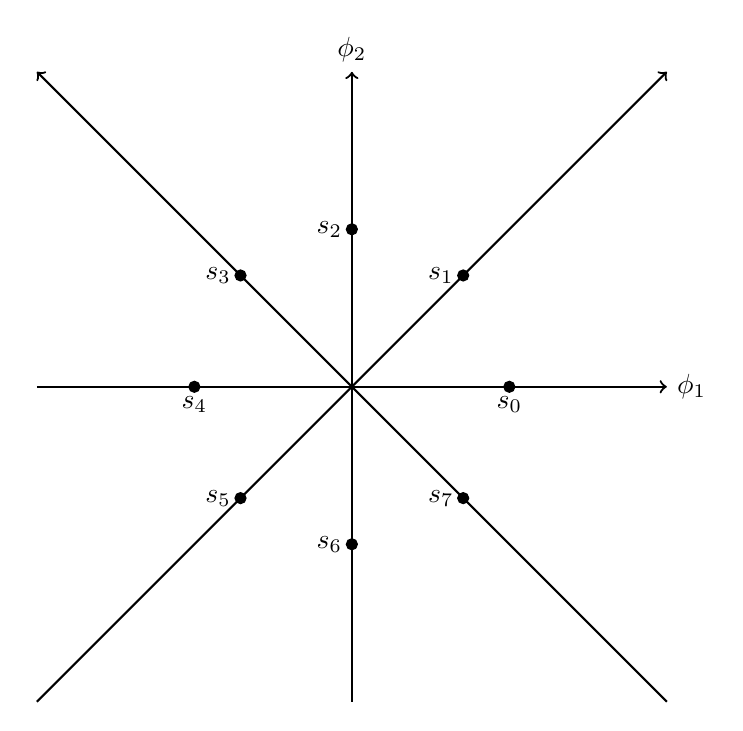
\begin{tikzpicture}

\draw[->,thick] (-4,0)--(4,0) node[right]{$\phi_1$};
\draw[->,thick] (0,-4)--(0,4) node[above]{$\phi_2$};
\draw[->,thick] (-4,-4)--(4,4) node[right]{};
\draw[->,thick] (4,-4)--(-4,4) node[above]{};

\filldraw[black] (2,0) circle (2pt) node[below] {$s_0$} ;
\filldraw[black] (1.414,1.414) circle (2pt) node[left] {$s_1$} ;
\filldraw[black] (0,2) circle (2pt) node[left] {$s_2$} ;
\filldraw[black] (-1.414,1.414) circle (2pt) node[left] {$s_3$} ;
\filldraw[black] (-2,0) circle (2pt) node[below] {$s_4$} ;
\filldraw[black] (-1.414,-1.414) circle (2pt) node[left] {$s_5$} ;
\filldraw[black] (0,-2) circle (2pt) node[left] {$s_6$} ;
\filldraw[black] (1.414,-1.414) circle (2pt) node[left] {$s_7$} ;


\end{tikzpicture}
}
\label{fig:ee18btech11012_fig1}
\caption{Constellation diagram}
\end{figure}


\item Encoding

$s_0$ denote bits 000, $s_1$ denote bits 001, $s_2$ denote bits 011,$s_3$ denote bits 010,$s_4$ denote bits 110,$s_5$ denote bits 111,$s_6$ denote bits 101,$s_7$ denote bits 100.
\begin{figure}[!ht]
                \resizebox{\columnwidth}{!}{%%%%%%%%%%%%%%%%%%%%%%%%%%%%%%%%%%%%%%%%%%%%%%%%%%%%%%%%%%%%%%%%%%%%%%
%%                                                                  %%
%%  This is the header of a LaTeX2e file exported from Gnumeric.    %%
%%                                                                  %%
%%  This file can be compiled as it stands or included in another   %%
%%  LaTeX document. The table is based on the longtable package so  %%
%%  the longtable options (headers, footers...) can be set in the   %%
%%  preamble section below (see PRAMBLE).                           %%
%%                                                                  %%
%%  To include the file in another, the following two lines must be %%
%%  in the including file:                                          %%
%%        \def\inputGnumericTable{}                                 %%
%%  at the beginning of the file and:                               %%
%%        \input{name-of-this-file.tex}                             %%
%%  where the table is to be placed. Note also that the including   %%
%%  file must use the following packages for the table to be        %%
%%  rendered correctly:                                             %%
%%    \usepackage[latin1]{inputenc}                                 %%
%%    \usepackage{color}                                            %%
%%    \usepackage{array}                                            %%
%%    \usepackage{longtable}                                        %%
%%    \usepackage{calc}                                             %%
%%    \usepackage{multirow}                                         %%
%%    \usepackage{hhline}                                           %%
%%    \usepackage{ifthen}                                           %%
%%  optionally (for landscape tables embedded in another document): %%
%%    \usepackage{lscape}                                           %%
%%                                                                  %%
%%%%%%%%%%%%%%%%%%%%%%%%%%%%%%%%%%%%%%%%%%%%%%%%%%%%%%%%%%%%%%%%%%%%%%



%%  This section checks if we are begin input into another file or  %%
%%  the file will be compiled alone. First use a macro taken from   %%
%%  the TeXbook ex 7.7 (suggestion of Han-Wen Nienhuys).            %%
\def\ifundefined#1{\expandafter\ifx\csname#1\endcsname\relax}


%%  Check for the \def token for inputed files. If it is not        %%
%%  defined, the file will be processed as a standalone and the     %%
%%  preamble will be used.                                          %%
\ifundefined{inputGnumericTable}

%%  We must be able to close or not the document at the end.        %%
	\def\gnumericTableEnd{\end{document}}


%%%%%%%%%%%%%%%%%%%%%%%%%%%%%%%%%%%%%%%%%%%%%%%%%%%%%%%%%%%%%%%%%%%%%%
%%                                                                  %%
%%  This is the PREAMBLE. Change these values to get the right      %%
%%  paper size and other niceties.                                  %%
%%                                                                  %%
%%%%%%%%%%%%%%%%%%%%%%%%%%%%%%%%%%%%%%%%%%%%%%%%%%%%%%%%%%%%%%%%%%%%%%

	\documentclass[12pt%
			  %,landscape%
                    ]{report}
       \usepackage[latin1]{inputenc}
       \usepackage{fullpage}
       \usepackage{color}
       \usepackage{array}
       \usepackage{longtable}
       \usepackage{calc}
       \usepackage{multirow}
       \usepackage{hhline}
       \usepackage{ifthen}

	\begin{document}


%%  End of the preamble for the standalone. The next section is for %%
%%  documents which are included into other LaTeX2e files.          %%
\else

%%  We are not a stand alone document. For a regular table, we will %%
%%  have no preamble and only define the closing to mean nothing.   %%
    \def\gnumericTableEnd{}

%%  If we want landscape mode in an embedded document, comment out  %%
%%  the line above and uncomment the two below. The table will      %%
%%  begin on a new page and run in landscape mode.                  %%
%       \def\gnumericTableEnd{\end{landscape}}
%       \begin{landscape}


%%  End of the else clause for this file being \input.              %%
\fi

%%%%%%%%%%%%%%%%%%%%%%%%%%%%%%%%%%%%%%%%%%%%%%%%%%%%%%%%%%%%%%%%%%%%%%
%%                                                                  %%
%%  The rest is the gnumeric table, except for the closing          %%
%%  statement. Changes below will alter the table's appearance.     %%
%%                                                                  %%
%%%%%%%%%%%%%%%%%%%%%%%%%%%%%%%%%%%%%%%%%%%%%%%%%%%%%%%%%%%%%%%%%%%%%%

\providecommand{\gnumericmathit}[1]{#1} 
%%  Uncomment the next line if you would like your numbers to be in %%
%%  italics if they are italizised in the gnumeric table.           %%
%\renewcommand{\gnumericmathit}[1]{\mathit{#1}}
\providecommand{\gnumericPB}[1]%
{\let\gnumericTemp=\\#1\let\\=\gnumericTemp\hspace{0pt}}
 \ifundefined{gnumericTableWidthDefined}
        \newlength{\gnumericTableWidth}
        \newlength{\gnumericTableWidthComplete}
        \newlength{\gnumericMultiRowLength}
        \global\def\gnumericTableWidthDefined{}
 \fi
%% The following setting protects this code from babel shorthands.  %%
 \ifthenelse{\isundefined{\languageshorthands}}{}{\languageshorthands{english}}
%%  The default table format retains the relative column widths of  %%
%%  gnumeric. They can easily be changed to c, r or l. In that case %%
%%  you may want to comment out the next line and uncomment the one %%
%%  thereafter                                                      %%
\providecommand\gnumbox{\makebox[0pt]}
%%\providecommand\gnumbox[1][]{\makebox}

%% to adjust positions in multirow situations                       %%
\setlength{\bigstrutjot}{\jot}
\setlength{\extrarowheight}{\doublerulesep}

%%  The \setlongtables command keeps column widths the same across  %%
%%  pages. Simply comment out next line for varying column widths.  %%
\setlongtables

\setlength\gnumericTableWidth{%
	71pt+%
	53pt+%
	69pt+%
0pt}
\def\gumericNumCols{3}
\setlength\gnumericTableWidthComplete{\gnumericTableWidth+%
         \tabcolsep*\gumericNumCols*2+\arrayrulewidth*\gumericNumCols}
\ifthenelse{\lengthtest{\gnumericTableWidthComplete > \linewidth}}%
         {\def\gnumericScale{\ratio{\linewidth-%
                        \tabcolsep*\gumericNumCols*2-%
                        \arrayrulewidth*\gumericNumCols}%
{\gnumericTableWidth}}}%
{\def\gnumericScale{1}}

%%%%%%%%%%%%%%%%%%%%%%%%%%%%%%%%%%%%%%%%%%%%%%%%%%%%%%%%%%%%%%%%%%%%%%
%%                                                                  %%
%% The following are the widths of the various columns. We are      %%
%% defining them here because then they are easier to change.       %%
%% Depending on the cell formats we may use them more than once.    %%
%%                                                                  %%
%%%%%%%%%%%%%%%%%%%%%%%%%%%%%%%%%%%%%%%%%%%%%%%%%%%%%%%%%%%%%%%%%%%%%%

\ifthenelse{\isundefined{\gnumericColA}}{\newlength{\gnumericColA}}{}\settowidth{\gnumericColA}{\begin{tabular}{@{}p{71pt*\gnumericScale}@{}}x\end{tabular}}
\ifthenelse{\isundefined{\gnumericColB}}{\newlength{\gnumericColB}}{}\settowidth{\gnumericColB}{\begin{tabular}{@{}p{53pt*\gnumericScale}@{}}x\end{tabular}}
\ifthenelse{\isundefined{\gnumericColC}}{\newlength{\gnumericColC}}{}\settowidth{\gnumericColC}{\begin{tabular}{@{}p{69pt*\gnumericScale}@{}}x\end{tabular}}

\begin{tabular}[c]{%
	b{\gnumericColA}%
	b{\gnumericColB}%
	b{\gnumericColC}%
	}

%%%%%%%%%%%%%%%%%%%%%%%%%%%%%%%%%%%%%%%%%%%%%%%%%%%%%%%%%%%%%%%%%%%%%%
%%  The longtable options. (Caption, headers... see Goosens, p.124) %%
%	\caption{The Table Caption.}             \\	%
% \hline	% Across the top of the table.
%%  The rest of these options are table rows which are placed on    %%
%%  the first, last or every page. Use \multicolumn if you want.    %%

%%  Header for the first page.                                      %%
%	\multicolumn{3}{c}{The First Header} \\ \hline 
%	\multicolumn{1}{c}{colTag}	%Column 1
%	&\multicolumn{1}{c}{colTag}	%Column 2
%	&\multicolumn{1}{c}{colTag}	\\ \hline %Last column
%	\endfirsthead

%%  The running header definition.                                  %%
%	\hline
%	\multicolumn{3}{l}{\ldots\small\slshape continued} \\ \hline
%	\multicolumn{1}{c}{colTag}	%Column 1
%	&\multicolumn{1}{c}{colTag}	%Column 2
%	&\multicolumn{1}{c}{colTag}	\\ \hline %Last column
%	\endhead

%%  The running footer definition.                                  %%
%	\hline
%	\multicolumn{3}{r}{\small\slshape continued\ldots} \\
%	\endfoot

%%  The ending footer definition.                                   %%
%	\multicolumn{3}{c}{That's all folks} \\ \hline 
%	\endlastfoot
%%%%%%%%%%%%%%%%%%%%%%%%%%%%%%%%%%%%%%%%%%%%%%%%%%%%%%%%%%%%%%%%%%%%%%
\hhline{|-|-|-}
	 \multicolumn{1}{|p{\gnumericColA}|}%
	{\gnumericPB{\centering}\gnumbox{Symbol}}
	&\multicolumn{1}{p{\gnumericColB}|}%
	{\gnumericPB{\centering}\gnumbox{Gray Code}}
	&\multicolumn{1}{p{\gnumericColC}|}%
	{\gnumericPB{\centering}\gnumbox{Value}}
\\
\hhline{|---|}
	 \multicolumn{1}{|p{\gnumericColA}|}%
	{\gnumericPB{\centering}\gnumbox{$s_0$}}
	&\multicolumn{1}{p{\gnumericColB}|}%
	{\gnumericPB{\centering}\gnumbox{000}}
	&\multicolumn{1}{p{\gnumericColC}|}%
	{\gnumericPB{\centering}\gnumbox{\myvec{1\\0 }}}
\\
\hhline{|---|}
	 \multicolumn{1}{|p{\gnumericColA}|}%
	{\gnumericPB{\centering}\gnumbox{$s_1$}}
	&\multicolumn{1}{p{\gnumericColB}|}%
	{\gnumericPB{\centering}\gnumbox{001}}
	&\multicolumn{1}{p{\gnumericColC}|}%
	{\gnumericPB{\centering}\gnumbox{\myvec{\frac{1}{\sqrt{2}}\\\frac{1}{\sqrt{2}}}}}
\\
\hhline{|---|}
	 \multicolumn{1}{|p{\gnumericColA}|}%
	{\gnumericPB{\centering}\gnumbox{$s_2$}}
	&\multicolumn{1}{p{\gnumericColB}|}%
	{\gnumericPB{\centering}\gnumbox{011}}
	&\multicolumn{1}{p{\gnumericColC}|}%
	{\gnumericPB{\centering}\gnumbox{\myvec{0\\1}}}
\\
\hhline{|---|}
	 \multicolumn{1}{|p{\gnumericColA}|}%
	{\gnumericPB{\centering}\gnumbox{$s_3$}}
	&\multicolumn{1}{p{\gnumericColB}|}%
	{\gnumericPB{\centering}\gnumbox{010}}
	&\multicolumn{1}{p{\gnumericColC}|}%
	{\gnumericPB{\centering}\gnumbox{\myvec{\frac{-1}{\sqrt{2}}\\\frac{1}{\sqrt{2}}}}}
\\
\hhline{|---|}
	 \multicolumn{1}{|p{\gnumericColA}|}%
	{\gnumericPB{\centering}\gnumbox{$s_4$}}
	&\multicolumn{1}{p{\gnumericColB}|}%
	{\gnumericPB{\centering}\gnumbox{110}}
	&\multicolumn{1}{p{\gnumericColC}|}%
	{\gnumericPB{\centering}\gnumbox{\myvec{-1\\0}}}
\\
\hhline{|---|}
	 \multicolumn{1}{|p{\gnumericColA}|}%
	{\gnumericPB{\centering}\gnumbox{$s_5$}}
	&\multicolumn{1}{p{\gnumericColB}|}%
	{\gnumericPB{\centering}\gnumbox{111}}
	&\multicolumn{1}{p{\gnumericColC}|}%
	{\gnumericPB{\centering}\gnumbox{\myvec{\frac{-1}{\sqrt{2}}\\\frac{-1}{\sqrt{2}}}}}
\\
\hhline{|---|}
	 \multicolumn{1}{|p{\gnumericColA}|}%
	{\gnumericPB{\centering}\gnumbox{$s_6$}}
	&\multicolumn{1}{p{\gnumericColB}|}%
	{\gnumericPB{\centering}\gnumbox{101}}
	&\multicolumn{1}{p{\gnumericColC}|}%
	{\gnumericPB{\centering}\gnumbox{\myvec{0\\-1}}}
\\
\hhline{|---|}
	 \multicolumn{1}{|p{\gnumericColA}|}%
	{\gnumericPB{\centering}\gnumbox{$s_7$}}
	&\multicolumn{1}{p{\gnumericColB}|}%
	{\gnumericPB{\centering}\gnumbox{100}}
	&\multicolumn{1}{p{\gnumericColC}|}%
	{\gnumericPB{\centering}\gnumbox{\myvec{\frac{1}{\sqrt{2}}\\\frac{-1}{\sqrt{2}}}}}
\\
\hhline{|-|-|-|}
\end{tabular}


\ifthenelse{\isundefined{\languageshorthands}}{}{\languageshorthands{\languagename}}
\gnumericTableEnd
}
\label{fig:ee18btech11012_fig2}
\caption{Gray coding}
\end{figure}

\item Decoding



\begin{figure}[!ht]

                \resizebox{\columnwidth}{!}{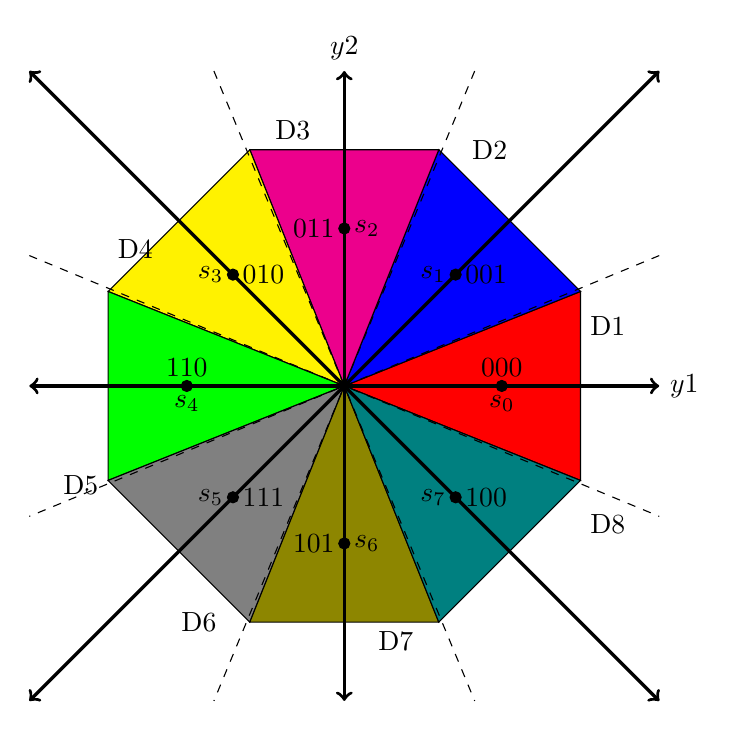
\begin{tikzpicture}
\draw[fill=red]  (0,0) -- (3,1.2) -- (3,-1.2) -- (0,0) -- cycle;
\draw[fill=blue]  (0,0) -- (1.2,3) -- (3,1.2) -- (0,0) -- cycle;
\draw[fill=magenta!100]  (0,0) -- (-1.2,3) -- (1.2,3) -- (0,0) -- cycle;
\draw[fill=yellow]  (0,0) -- (-1.2,3) -- (-3,1.2) -- (0,0) -- cycle;
\draw[fill=green]  (0,0) -- (-3,1.2) -- (-3,-1.2) -- (0,0) -- cycle;
\draw[fill=gray]  (0,0) -- (-3,-1.2) -- (-1.2,-3) -- (0,0) -- cycle;
\draw[fill=olive]  (0,0) -- (-1.2,-3) -- (1.2,-3) -- (0,0) -- cycle;
\draw[fill=teal]  (0,0) -- (1.2,-3) -- (3,-1.2) -- (0,0) -- cycle;
\draw[<->,very thick] (-4,0)--(4,0) node[right]{$y1$};
\draw[<->,very thick] (0,-4)--(0,4) node[above]{$y2$};
\draw[dashed] (4,1.656)--(-4,-1.656);
\draw[dashed] (1.656,4)--(-1.656,-4);
\draw[dashed] (-1.656,4)--(1.656,-4);
\draw[dashed] (-4,1.656)--(4,-1.656);
\draw[<->,very thick](-4,-4)--(4,4);
\draw[<->,very thick](-4,4)--(4,-4);

\filldraw[black] (2,0) circle (2pt) node[below] {$s_0$} node[above] {000};
\filldraw[black] (1.414,1.414) circle (2pt) node[left] {$s_1$} node[right] {001};
\filldraw[black] (0,2) circle (2pt) node[right] {$s_2$} node[left] {011};
\filldraw[black] (-1.414,1.414) circle (2pt) node[left] {$s_3$} node [right] {010};
\filldraw[black] (-2,0) circle (2pt) node[below] {$s_4$} node[above] {110};
\filldraw[black] (-1.414,-1.414) circle (2pt) node[left] {$s_5$} node[right] {111};
\filldraw[black] (0,-2) circle (2pt) node[right] {$s_6$} node[left] {101};
\filldraw[black] (1.414,-1.414) circle (2pt) node[left] {$s_7$} node [right] {100};

\foreach \coordinate/\label/\pos in {{(3,1)/D1/below right},{(1.5,3)/D2/right},{(-1,3)/D3/above right},{(-3,1.5)/D4/above right},{(-3,-1.5)/D5/above left},{(-1.5,-3)/D6/left},{(1,-3)/D7/below left},{(3,-2)/D8/above right}} \node[\pos] at \coordinate {\label};

\end{tikzpicture}
}

\label{fig:ee18btech11012_fig3}
\caption{decision regions}
	
\end{figure}

\textbf{\underline{Minimum distance Criterion}:}
\begin{align}
    \hat{s} = min \norm{\textbf{y} - \textbf{s}}
    \label{eq:ee18btech11012_eq1}
\end{align}
where \textbf{s} \in {$s_{0}$,$s_{1}$,$s_{2}$,.....$s_{M}$}\\
From eq.\ref{eq:ee18btech11012_eq1},\textbf{$s_{0}$} is chosen if
\begin{align}
    \norm{\textbf{y}-\textbf{$s_{0}$}}^2 < \norm{\textbf{y}-\textbf{$s_{1}$}}^2
\end{align}
\begin{align}
    \norm{\textbf{y}-\textbf{$s_{0}$}}^2 < \norm{\textbf{y}-\textbf{$s_{2}$}}^2
\end{align}
\begin{align}
    \norm{\textbf{y}-\textbf{$s_{0}$}}^2 < \norm{\textbf{y}-\textbf{$s_{3}$}}^2
\end{align}
\begin{align}
    \norm{\textbf{y}-\textbf{$s_{0}$}}^2 < \norm{\textbf{y}-\textbf{$s_{4}$}}^2
\end{align}
\begin{align}
    \norm{\textbf{y}-\textbf{$s_{0}$}}^2 < \norm{\textbf{y}-\textbf{$s_{5}$}}^2
\end{align}
\begin{align}
    \norm{\textbf{y}-\textbf{$s_{0}$}}^2 < \norm{\textbf{y}-\textbf{$s_{6}$}}^2
\end{align}
\begin{align}
    \norm{\textbf{y}-\textbf{$s_{0}$}}^2 < \norm{\textbf{y}-\textbf{$s_{7}$}}^2
\end{align}
Since $\norm{s_{i}}^2$ = $E_{s}$,the above conditions can be simplified to obtain the region
\begin{align}
    (s_{0}-s_{1})^Ty>0
\end{align}
\begin{align}
    (s_{0}-s_{2})^Ty>0
\end{align}
\begin{align}
    (s_{0}-s_{3})^Ty>0
\end{align}
\begin{align}
    (s_{0}-s_{4})^Ty>0
\end{align}
\begin{align}
    (s_{0}-s_{5})^Ty>0
\end{align}
\begin{align}
    (s_{0}-s_{6})^Ty>0
\end{align}
\begin{align}
    (s_{0}-s_{7})^Ty>0
\end{align}
Substituting the values of $s_{0}$,$s_{1}$,....$s_{7}$ in the above and eliminating $\sqrt{E_{s}}$,,the desired region is
\begin{align}
    \myvec{(1-\frac{1}{\sqrt{2}})\\\frac{-1}{\sqrt{2}}}^T\myvec{y_{1}\\y_{2}} > 0
\end{align}
\begin{align}
    \myvec{1\\-1}^T\myvec{y_{1}\\y_{2}} > 0
\end{align}
\begin{align}
    \myvec{(1+\frac{1}{\sqrt{2}})\\\frac{-1}{\sqrt{2}}}^T\myvec{y_{1}\\y_{2}} > 0
\end{align}
\begin{align}
    \myvec{1\\0}^T\myvec{y_{1}\\y_{2}} > 0
\end{align}
\begin{align}
    \myvec{(1+\frac{1}{\sqrt{2}})\\\frac{1}{\sqrt{2}}}^T\myvec{y_{1}\\y_{2}} > 0
\end{align}
\begin{align}
    \myvec{1\\1}^T\myvec{y_{1}\\y_{2}} > 0
\end{align}
\begin{align}
    \myvec{(1-\frac{1}{\sqrt{2}})\\\frac{1}{\sqrt{2}}}^T\myvec{y_{1}\\y_{2}} > 0
\end{align}
yielding \abs{y_{2}} < (\sqrt{2}-1)$y_{1}$ \\i.e.,Red region(D1) is detected at the receiver.
\\
Similarly,\\
From eq:\ref{eq:ee18btech11012_eq1}\\
For detecting $s_1$, $y_2-(\sqrt{2}+1)y_1<0$ and $y_2-(\sqrt{2}-1)y_1>0$.\\
$\Longleftrightarrow$ D2(blue) region is detected at receiver
\\
For detecting $s_2$,$y_2-(\sqrt{2}+1)y_1 >0$ and $y_2+(\sqrt{2}+1)y_1>0$\\$\Longleftrightarrow$ D3(pink) region at receiver. 
\\
For detecting $s_3$, $y_2+(\sqrt{2}-1)y_1>0$ and $y_2+(\sqrt{2}+1)y_1<0$.\\
$\Longleftrightarrow$ D4(yellow) region at receiver.
\\
For detecting $s_4$, $y_2+(\sqrt{2}-1)y_1<0$ and $y_2-(\sqrt{2}-1)y_1>0$.\\
$\Longleftrightarrow$ D5(green) region at receiver.
\\
For detecting $s_5$, $y_2-(\sqrt{2}+1)y_1>0$ and $y_2-(\sqrt{2}-1)y_1<0$.\\
$\Longleftrightarrow$ D6(grey) region at receiver.
\\
For detecting $s_6$, $y_2-(\sqrt{2}+1)y_1<0$ and $y_2+(\sqrt{2}+1)y_1<0$.\\
$\Longleftrightarrow$ D7(olive) region at receiver.
\\
For detecting $s_7$, $y_2+(\sqrt{2}-1)y_1<0$ and $y_2+(\sqrt{2}+1)y_1>0$.\\
$\Longleftrightarrow$ D8(teal) region at receiver.



\item The following code has simulation of 8PSK.
\begin{lstlisting}
 codes/ee18btech11012.py
\end{lstlisting}
\end{enumerate}
